% !TEX root = ../../Main.tex
\section{Portfolio: The Seven Models Combined}
\label{Section:Portfolio}

A trader would not run just one of these agents. They would run all seven. This is a different question from how each agent does alone. For a portfolio, what matters is not only what each component returns, but also whether the components lose money at the same time.

The seven published models are combined by giving each one a seventh of the capital at the start of the window, with no rebalancing afterwards. With $E_p(t)$ the equity of pair $p$ at time $t$, the portfolio is

\begin{equation}
V(t) = \frac{1}{7} \sum_{p} \frac{E_p(t)}{E_p(0)}
\label{Equation:Portfolio}
\end{equation}

By construction, the total return of such a portfolio is the mean of its components. The interesting part is therefore the risk, and not the return. \Cref{Tables:Portfolio} compares the portfolio with the average of the seven pairs taken separately.

% !TEX root = ../Main.tex
\begin{table}[htb!]
\centering
\footnotesize
\caption{The equal-weight portfolio of \Cref{Equation:Portfolio} against the average of its seven components. Return is the same by construction, so the whole effect is on risk.}
\label{Tables:Portfolio}
\begin{tabular}{@{}lrrl@{}}
\toprule
\textbf{Measure} & \textbf{Portfolio} & \textbf{Mean of the seven} & \textbf{Effect} \\
\midrule
Total return & $+91.3\%$ & $+91.3\%$ & Equal by construction \\
Annualised return & $+6.07\%$ & $+6.07\%$ & Equal by construction \\
\addlinespace
Maximum drawdown & $\mathbf{15.9\%}$ & $34.5\%$ & More than halved \\
Sharpe ratio & $\mathbf{0.632}$ & $0.451$ & Above all but USD/CHF \\
Sortino ratio & $0.906$ & $0.685$ & Improved \\
Calmar ratio & $0.381$ & $0.194$ & Nearly doubled \\
Sterling ratio & $1.059$ & $0.670$ & Improved \\
\addlinespace
Mean correlation & \multicolumn{2}{c}{$+0.062$ across all 21 pairings} & Close to independent \\
\bottomrule
\end{tabular}
\end{table}

\Cref{Figure:PortfolioEquity} plots the portfolio against its components. The maximum drawdown falls from an average of $34.5\%$ to $15.9\%$. The Sharpe ratio rises from an average of $0.451$ to $0.632$, which is above every single pair except USD/CHF. The portfolio gives the same return with less than half the worst loss.

\begin{figure}[htb!]
\centering
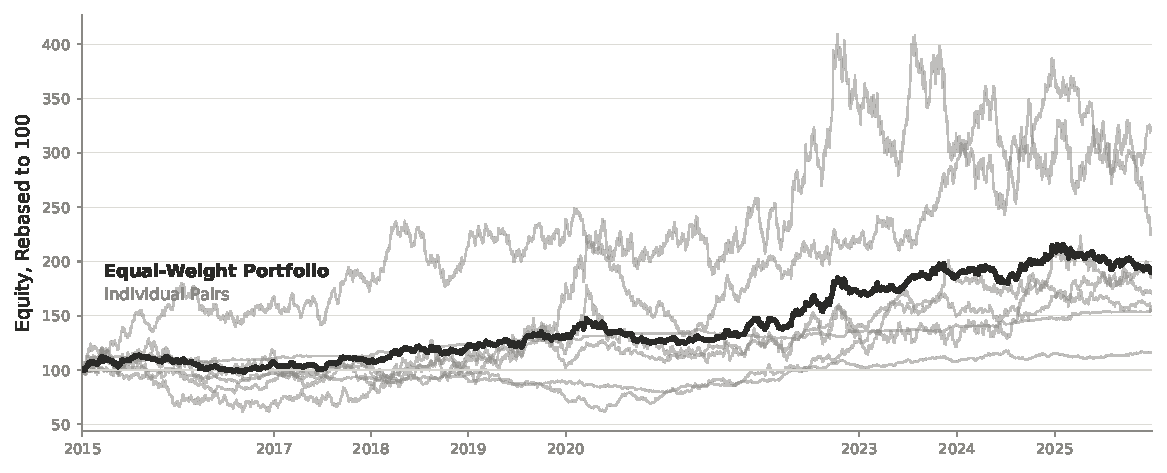
\includegraphics[width=\textwidth]{Images/PortfolioEquity.pdf}
\caption{The equal-weight portfolio against its seven components, all rebased to 100. The portfolio is smoother than any component because the components do not fall together.}
\label{Figure:PortfolioEquity}
\end{figure}

\Cref{Figure:Correlation} shows the reason. The mean correlation between the daily returns of any two of the seven models is $+0.062$, and no pair of models is above $+0.46$. Three pairings are negative. The seven agents were trained by the same procedure on seven instruments that are themselves correlated, since all of them have the US Dollar on one side. Even so, their profits and losses come at different times. This follows from the design. Each agent learned the timing of its own market, so the agents share a method but not a position.

\begin{figure}[htb!]
\centering
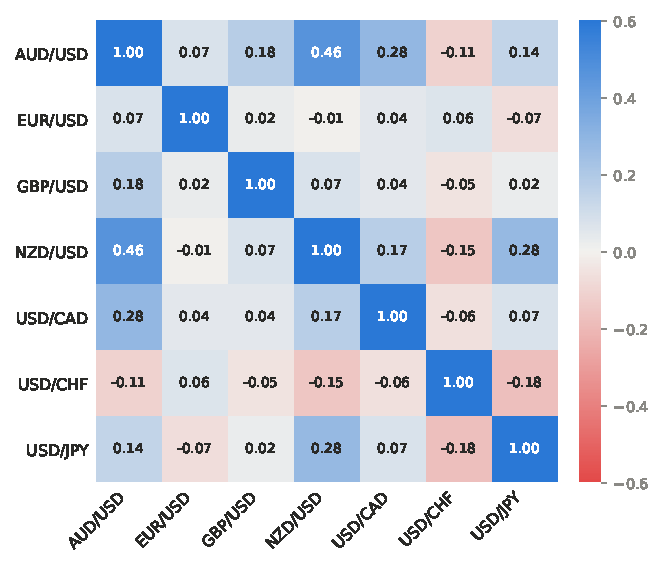
\includegraphics[width=0.68\textwidth]{Images/Correlation.pdf}
\caption{Correlation between the daily returns of the seven agents over the evaluation window. The mean of the off-diagonal entries is $+0.062$.}
\label{Figure:Correlation}
\end{figure}

\subsection{Does the Result Depend on the Position Sizes?}

As \Cref{Section:EvaluationProtocol} states, the seven models do not all run at the same position size. The portfolio above is therefore the combination as published, and it is not built on a common risk level. It is fair to ask whether this choice produces the result. The question can be checked directly.

Position size is proportional to the account balance. Multiplying the risk fraction by a constant therefore multiplies every position, and so every per-step return, by the same constant. A common-risk version can be built by rescaling each component's returns to the level it would have run at, and compounding them again. This ignores the rounding of volumes to the broker's step and any margin limit. It is an approximation and not a new run, but it is close enough to answer the question. \Cref{Tables:CommonRisk} gives both versions.

% !TEX root = ../Main.tex
\begin{table}[htb!]
\centering
\footnotesize
\caption{The equal-weight portfolio as published, against a version in which every component runs at a common risk level. The common-risk version is built by rescaling each component's per-step returns. This is exact for a strategy whose position size is proportional to balance, but it ignores volume rounding. The two differ little, so the diversification result does not depend on how positions are sized.}
\label{Tables:CommonRisk}
\begin{tabular}{@{}lrrr@{}}
\toprule
\textbf{Measure} & \textbf{As Published} & \textbf{Common Risk} & \textbf{Difference} \\
\midrule
Total return & $+91.3\%$ & $+91.6\%$ & $+0.3$ pp \\
Annualised return & $+6.07\%$ & $+6.09\%$ & $+0.02$ pp \\
Sharpe ratio & $0.632$ & $0.608$ & $-0.024$ \\
Sortino ratio & $0.906$ & $0.866$ & $-0.040$ \\
Calmar ratio & $0.381$ & $0.320$ & $-0.061$ \\
Maximum drawdown & $15.9\%$ & $19.0\%$ & $+3.1$ pp \\
\bottomrule
\end{tabular}
\end{table}

The two portfolios are almost the same. Total return moves from $+91.3\%$ to $+91.6\%$, the Sharpe ratio from $0.632$ to $0.608$, and the maximum drawdown from $15.9\%$ to $19.0\%$. The common-risk version is slightly worse on risk, as expected. Putting USD/JPY at the same risk level as the others makes its positions five times larger and takes its own maximum drawdown to roughly $80\%$. At a seventh of the capital, the portfolio absorbs even that. The conclusion of this section therefore does not depend on how the positions are sized. It depends on the correlation structure of the models, which sizing does not change.

Two limits apply to this result. As \Cref{Section:EvaluationProtocol} states, the components do not all run at the same position size. The portfolio is therefore the combination as published, and not a risk-parity allocation. Making the sizes equal would change the weights, but not the correlation structure that produces the benefit. Also, the portfolio shares the weakness of its components. In the held-out year of \Cref{Section:OutOfSample} it returns $-9.8\%$, better than five of the seven pairs and worse than two. This is what an average should do when most of its components fall together for a shared reason.